\begin{abstract}

Composite materials or prepregs are terms that have increasingly found their
way into the day to day reality around the aerospace industry in particular, but
in day to day life in general. They have kickstarted a technological revolution
within the sector unlike anything seen in the last decades.\\

The use of glass, carbon, aramid… reinforced polymers, has become mainstream
in aerospace products during the last decade. As an example of these, the two
biggest aircraft manufacturers, Boeing and Airbus, have introduced in this decade
two wide body airplanes that extensively use CFRP as main material for their fuselage,
wings, tail surfaces, etc.\\

With all this in mind, there is no doubt that the industry has had to keep up
to this technological leap, especially in the field of prepreg manufacturing.
Thus, this paper reviews these techniques and processes, with an insight on the
recent developments in prepreg part manufacturing.\\

\end{abstract}

\section{Introduction}

Prepregs are kind of composite material configuration in which the reinforcement
is already preimpregnated (hence the name) with the matrix. I other words, fibers
are embedded in the matrix beforehand by the manufacturer, unlike a bare fiber
fabric presentation with a future resin infusion.

The matrix selection is not constrained to a particular nature, but as a matter
of fact, thermoset options widely outweigh thermoplastics. The most popular choice
is epoxy resin based matrices.

\begin{figure}[h]
	\centering
	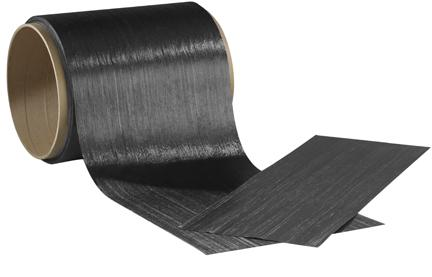
\includegraphics[width=0.6\textwidth]{img/prepreg_roll.jpg}
	\caption[Carbon fiber prepreg roll]{Commercial example of a carbon fiber prepreg roll.
	Photo credit: Zoltek Corp.}
	\label{fig:prepreg_roll}
\end{figure}

Interestingly, prepregs are not cured when delivered, otherwise it would not be
possible to conform to the desired shape. To avoid the resin curing while having
it incorporated in the composite beforehand, a staging process is applied. It
basically halts the chemical reaction associated to curing, leaving it at the early
stages, with a consistence valid for the embedding into the reinforcement.\\

hen, they must be stored in a chilled facility in order to stop the chemical
reaction from completing. Usually the storage temperature is set at around -18 ºC,
having roughly a year of shelf life under these circumstances \cite{https://www.sciencedirect.com/science/article/pii/S2212827117311800}.\\

\subsection{Advantages and disadvantages}

To establish a fair comparison, prepregs must be faced with its closest, readily
available alternative, uni/bidirectional reinforcement fabric with later matrix
infusion. As:\\

\begin{itemize}
	\item Prepreg have higher fiber to weight ratio than the alternative fabric.
	\item Lower void presence in the final product, yielding higher mechanical properties.
	\item Supplied by a manufacturer, it is a final product, certificated and
	backed by company. Therefore, the final cured product is virtually the same,
	always. In the other case, worker’s craftsmanship plays a bigger role in
	manufacturing, leading to potential deviations and errors.
	\item As a result of the previous condition, faster and more straight
	forward inspection and quality checks.
\end{itemize}

As for the disadvantages:

\begin{itemize}
	\item Prepregs must be stored in colds rooms. This represents an additional
	expense both for the manufacturer and the final user.
	\item In general terms, expensive and complex autoclaves (ovens applying
	both pressure and heat) are required for prepreg curing.
	\item Higher overall cost.
\end{itemize}

\subsection{Historical evolution}

Composites, namely combinations of thermoplastic/thermoset matrices with fiber
(glass and carbon) reinforcements, saw their inception, development and first
introduction in the aerospace field in the 60s. As for prepregs, their usage fell
behind of conventional laid up fabric.\\

Initial projects involved experimental vehicles, such fighter aircraft. This low
volume and pioneering production went hand in hand with manual placement of fiber
fabric layers. As production volume increased, moving also to series production,
together with the advent of computer controlled machines, prepregs began taking
ever increasing share of the market.\\

Nowadays composites have penetrated almost all fields within the aerospace industry.
Aircraft, be it commercial or general aviation ones, have several key components
manufactured in prepreg composites, mainly CFRP and GFRP. Advanced and efficient
prepreg placing processes such Automatic Tape Laying allow for the production
of large structures like wing skins, reducing time and cost.\\

\section{Fields of applications of prepreg materials}

\subsection{Space applications}

\section{Aeronautical applications}

The aeronautical industry is starting to introduce the use of composite materials
and reinforced plastic. During the past 20 years its use has become widely extended
in the manufacture of aircrafts and nowadays lot of parts of them are made by composites.
This sector is, every year, demanding more composites in order to meet its needs
to reduce weight, save costs and improve manufacturing times. The composite industries
is developing new methods to satisfy this needs, and many of these are based on
out-of-autoclave processes. These are faster than the traditional ones, allowing
big savings in operational costs. Some analysts are projecting that in the next
5 years there will be an increase in the global composite market for aerospace
applications of  33\% giving a total production of 43.5 million kg. \cite{2}

Another way to see the change in the aerospace industry, which is continuously
moving to composite material solutions, is analyzing the materials in which are
manufactured a series of commercial aircraft, for example, in the figure [2] is
shown the Boeing famous airplanes, where it can be observed a clear trend to use
more composites in the last decades\cite{3}.
[3] Xuesong Zhang, Yongjun Chen, Junling Hu. Recent advantages in development in aerospace materials

\begin{figure}[h]
	\centering
	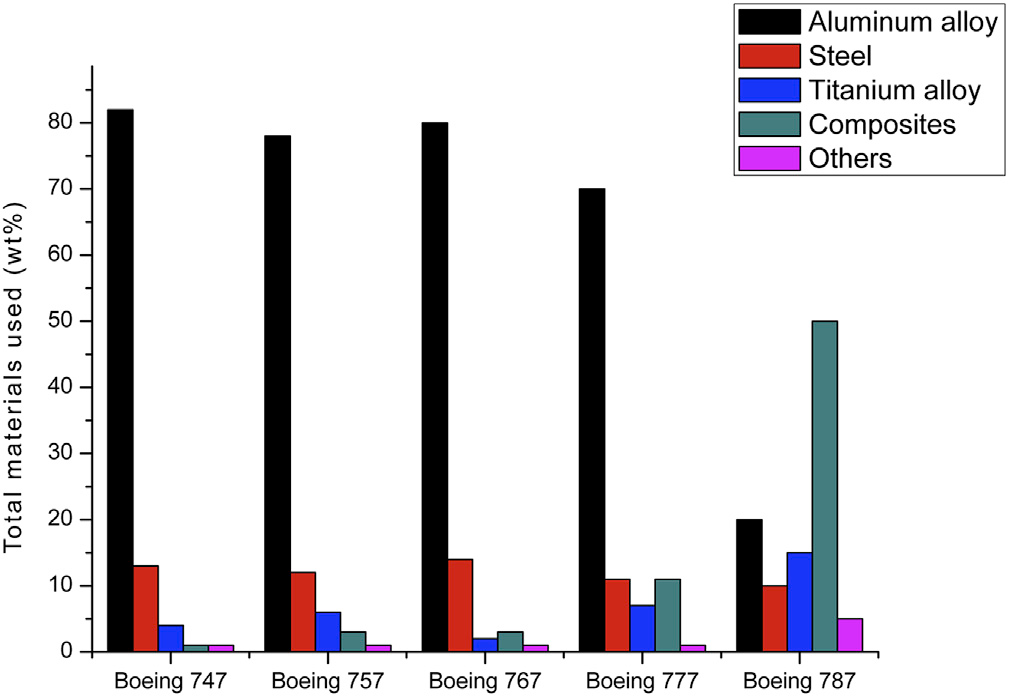
\includegraphics[width=0.8\textwidth]{img/boeing_aircrafts.png}
	\caption[Carbon fiber prepreg roll]{Evolution of the
	series of Boeing commercial aircrafts in terms of the materials used in
	its manufacture, showing a clear increase in composite materials solutions
	in the lasts models, specially in the last Boeing 787. \cite{3}}
	\label{fig:prepreg_roll}
\end{figure}
